%\documentclass[11pt]{paper}
%\usepackage{palatino}
%\usepackage{amsfonts,amsmath,amssymb}
%% \usepackage{graphicx}
%
%\usepackage{listings}
%\usepackage{textcomp}
%\usepackage{color}
%
%\definecolor{dkgreen}{rgb}{0,0.6,0}
%\definecolor{gray}{rgb}{0.5,0.5,0.5}
%\definecolor{mauve}{rgb}{0.58,0,0.82}
%
%\lstset{frame=tb,
%  language=R,
%  aboveskip=3mm,
%  belowskip=3mm,
%  showstringspaces=false,
%  columns=flexible,
%  basicstyle={\small\ttfamily},
%  numbers=none,
%  numberstyle=\tiny\color{gray},
%  keywordstyle=\color{blue},
%  commentstyle=\color{dkgreen},
%  stringstyle=\color{mauve},
%  breaklines=true,
%  breakatwhitespace=true,
%  tabsize=3
%}
%
%
%
%\ifx\pdftexversion\undefined
%    \usepackage[dvips]{graphicx}
%\else
%    \usepackage[pdftex]{graphicx}
%    \usepackage{epstopdf}
%    \epstopdfsetup{suffix=}
%\fi
%
%\usepackage{subfig}
%
%\begin{document}
%
%%%%%%%%%%%%%%%%%%%%%%%%%%%%%%%%%%%%%%%%%
%% Problem Set 6
%%%%%%%%%%%%%%%%%%%%%%%%%%%%%%%%%%%%%%%%%
%
%\pagestyle{empty}
%{\noindent\bf Spring 2023 \hfill Brandon~Parmanand}
%\vskip 16pt
%\centerline{\bf University of Central Florida}
%\centerline{\bf College of Business}
%\vskip 16pt
%\centerline{\bf QMB 6911}
%\centerline{\bf Capstone Project in Business Analytics}
%\vskip 10pt
%\centerline{\bf Solutions:  Problem Set \#6}
%\vskip 32pt
%\noindent
%
%\section{Data Description}
%
%This analysis follows the script \texttt{PS6.R} to produce a more accurate model for House prices with the data from \texttt{HomeSales.dat} in the \texttt{Data} folder. 
%
%
I will first estimate a model with the entire sampeles, including both rental and owner occupied. Then I will consider exclusions of insignificant variables from the full model. 
This approach allows for exclusion of possibly irrelevant variables and avoids excluding any relevant variables. 


%%%%%%%%%%%%%%%%%%%%%%%%%%%%%%%%%%%%%%%%
% Choosing the Dependent Variable
%%%%%%%%%%%%%%%%%%%%%%%%%%%%%%%%%%%%%%%%


\pagebreak
\section{Choosing the Dependent Variable}

Before we begin, I review the evidence for the suitability of the 
dependent variable without transformation
and compare that with the logarithmic transformation. 
Although, in this case, this decision is fairly clearly made by plotting the dependent variable alone, 
in many cases, the decision is not so clear and other forms
of evidence can be considered once building a model. 


\subsection{Univariate Analysis}

Figure \ref{fig:hist_price} shows a histogram of home prices.
This is a skewed distribution, which might influence the
estimates of parameters in the model so I will plot a histogram of the log of home prices.


\begin{figure}[h!]
  \centering
  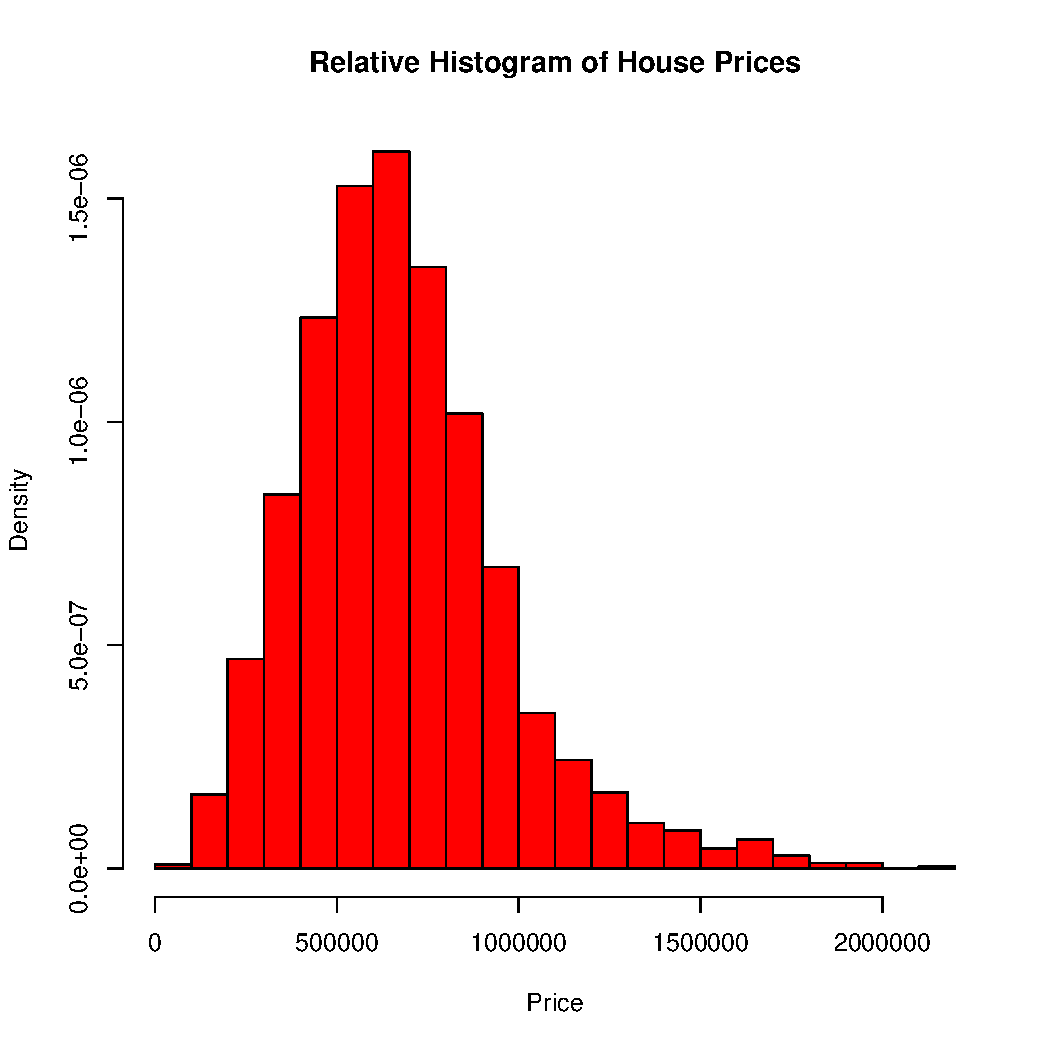
\includegraphics[scale = 0.5, keepaspectratio=true]{../Figures/hist_price}
  \caption{Histogram of House Prices} \label{fig:hist_price}
\end{figure}



\pagebreak
As a comparison, Figure \ref{fig:hist_log_price} shows the histogram of the natural logarithm of
price.

\begin{figure}[h!]
  \centering
  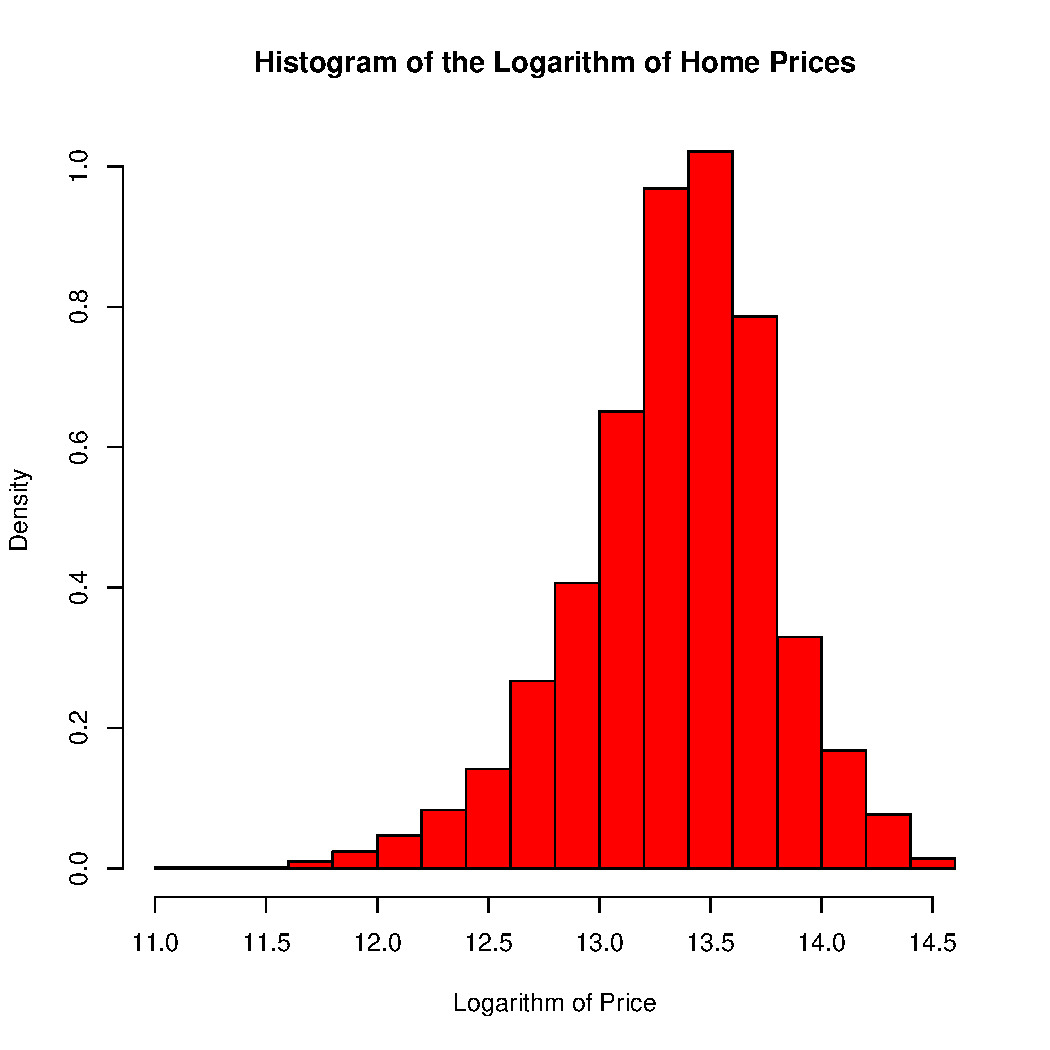
\includegraphics[scale = 0.5, keepaspectratio=true]{../Figures/hist_log_price}
  \caption{Histogram of the Logarithm of Tractor Prices} \label{fig:hist_log_price}
\end{figure}




%%%%%%%%%%%%%%%%%%%%%%%%%%%%%%%%%%%%%%%%
% Linear Regression Models
%%%%%%%%%%%%%%%%%%%%%%%%%%%%%%%%%%%%%%%%


\pagebreak
\subsection{Linear Regression Models of House Prices}


Here I build a regression model with all the variables and price and also another model with the natural logarithm prices.


\begin{table}
\begin{center}
\begin{tabular}{l c c}
\hline
 & Model 1 & Model 2 \\
\hline
(Intercept)       & $-13493752.25309^{***}$ & $-9.86780^{***}$ \\
                  & $(601281.58476)$        & $(0.84272)$      \\
YearBuilt         & $6615.49321^{***}$      & $0.01084^{***}$  \\
                  & $(298.74438)$           & $(0.00042)$      \\
NumBeds           & $92548.13460^{***}$     & $0.13122^{***}$  \\
                  & $(8006.80651)$          & $(0.01122)$      \\
NumBaths          & $26490.99054^{**}$      & $0.07083^{***}$  \\
                  & $(8377.76428)$          & $(0.01174)$      \\
FloorSpace        & $38.40785$              & $0.00002$        \\
                  & $(30.86097)$            & $(0.00004)$      \\
LotSize           & $21.54593^{***}$        & $0.00003^{***}$  \\
                  & $(2.90062)$             & $(0.00000)$      \\
HasGarage         & $130010.15275^{***}$    & $0.28206^{***}$  \\
                  & $(18873.47333)$         & $(0.02645)$      \\
HasEnclPatio      & $27910.39331^{***}$     & $0.05541^{***}$  \\
                  & $(8461.30634)$          & $(0.01186)$      \\
HasSecGate        & $155859.26108^{***}$    & $0.18598^{***}$  \\
                  & $(12498.19417)$         & $(0.01752)$      \\
HasPool           & $72977.97398^{***}$     & $0.07524^{**}$   \\
                  & $(17000.27998)$         & $(0.02383)$      \\
TransitScore      & $36115.28316^{***}$     & $0.06513^{***}$  \\
                  & $(1525.51010)$          & $(0.00214)$      \\
SchoolScore       & $954.30361$             & $0.00913^{***}$  \\
                  & $(1883.35880)$          & $(0.00264)$      \\
TypeOfBuyerRental & $80428.21155^{***}$     & $0.10219^{***}$  \\
                  & $(11282.76745)$         & $(0.01581)$      \\
\hline
R$^2$             & $0.59589$               & $0.67214$        \\
Adj. R$^2$        & $0.59392$               & $0.67055$        \\
Num. obs.         & $2473$                  & $2473$           \\
\hline
\multicolumn{3}{l}{\scriptsize{$^{***}p<0.001$; $^{**}p<0.01$; $^{*}p<0.05$}}
\end{tabular}
\caption{Linear and Logarithmic Models of House Prices}
\label{tab:reg_price_w_log}
\end{center}
\end{table}


The results of Model 1 and Model 2 in Table \ref{tab:reg_price_w_log}
shows the effect of the variables on the dollar price of the
home prices and natural logarithm of . 

From the R squared value, natural log model (Model 2) is a better model to use.


%%%%%%%%%%%%%%%%%%%%%%%%%%%%%%%%%%%%%%%%
\clearpage
\section{Model Specification}
%%%%%%%%%%%%%%%%%%%%%%%%%%%%%%%%%%%%%%%%

\subsection{Variable Reduction}

Next, I can refine the model by removing some explanatory variables that do not have string predictive value. 
The first candidates are those with coefficients that are not statistically significant. 
The results in Table \ref{tab:reg_reduction} are conducted using the natural logarithm prices as we concluded from the previous analysis.


\begin{table}
\begin{center}
\begin{tabular}{l c c c c c}
\hline
 & Model 1 & Model 2 & Model 3 & Model 4 & Model 5 \\
\hline
(Intercept)       & $-9.8678^{***}$ & $-9.8544^{***}$ & $-9.8423^{***}$ & $-9.8162^{***}$ & $-9.7645^{***}$ \\
                  & $(0.8427)$      & $(0.8420)$      & $(0.8438)$      & $(0.8477)$      & $(0.8489)$      \\
TypeOfBuyerRental & $0.1022^{***}$  & $0.1022^{***}$  & $0.1000^{***}$  & $0.0926^{***}$  & $0.0886^{***}$  \\
                  & $(0.0158)$      & $(0.0158)$      & $(0.0158)$      & $(0.0158)$      & $(0.0158)$      \\
YearBuilt         & $0.0108^{***}$  & $0.0108^{***}$  & $0.0108^{***}$  & $0.0108^{***}$  & $0.0108^{***}$  \\
                  & $(0.0004)$      & $(0.0004)$      & $(0.0004)$      & $(0.0004)$      & $(0.0004)$      \\
NumBeds           & $0.1312^{***}$  & $0.1344^{***}$  & $0.1386^{***}$  & $0.1473^{***}$  & $0.1498^{***}$  \\
                  & $(0.0112)$      & $(0.0085)$      & $(0.0084)$      & $(0.0082)$      & $(0.0082)$      \\
NumBaths          & $0.0708^{***}$  & $0.0722^{***}$  & $0.0749^{***}$  & $0.0783^{***}$  & $0.0774^{***}$  \\
                  & $(0.0117)$      & $(0.0113)$      & $(0.0113)$      & $(0.0114)$      & $(0.0114)$      \\
FloorSpace        & $0.0000$        &                 &                 &                 &                 \\
                  & $(0.0000)$      &                 &                 &                 &                 \\
LotSize           & $0.0000^{***}$  & $0.0000^{***}$  & $0.0000^{***}$  & $0.0000^{***}$  & $0.0000^{***}$  \\
                  & $(0.0000)$      & $(0.0000)$      & $(0.0000)$      & $(0.0000)$      & $(0.0000)$      \\
HasGarage         & $0.2821^{***}$  & $0.2902^{***}$  & $0.2953^{***}$  & $0.3015^{***}$  & $0.2978^{***}$  \\
                  & $(0.0265)$      & $(0.0185)$      & $(0.0184)$      & $(0.0185)$      & $(0.0185)$      \\
HasEnclPatio      & $0.0554^{***}$  & $0.0553^{***}$  & $0.0579^{***}$  &                 &                 \\
                  & $(0.0119)$      & $(0.0119)$      & $(0.0119)$      &                 &                 \\
HasSecGate        & $0.1860^{***}$  & $0.1864^{***}$  & $0.1927^{***}$  & $0.1880^{***}$  & $0.1855^{***}$  \\
                  & $(0.0175)$      & $(0.0175)$      & $(0.0174)$      & $(0.0175)$      & $(0.0175)$      \\
HasPool           & $0.0752^{**}$   & $0.0752^{**}$   & $0.0739^{**}$   & $0.0725^{**}$   &                 \\
                  & $(0.0238)$      & $(0.0238)$      & $(0.0239)$      & $(0.0240)$      &                 \\
TransitScore      & $0.0651^{***}$  & $0.0651^{***}$  & $0.0641^{***}$  & $0.0652^{***}$  & $0.0653^{***}$  \\
                  & $(0.0021)$      & $(0.0021)$      & $(0.0021)$      & $(0.0021)$      & $(0.0021)$      \\
SchoolScore       & $0.0091^{***}$  & $0.0090^{***}$  &                 &                 &                 \\
                  & $(0.0026)$      & $(0.0026)$      &                 &                 &                 \\
\hline
R$^2$             & $0.6721$        & $0.6721$        & $0.6705$        & $0.6674$        & $0.6661$        \\
Adj. R$^2$        & $0.6705$        & $0.6707$        & $0.6692$        & $0.6661$        & $0.6650$        \\
Num. obs.         & $2473$          & $2473$          & $2473$          & $2473$          & $2473$          \\
\hline
\multicolumn{6}{l}{\scriptsize{$^{***}p<0.001$; $^{**}p<0.01$; $^{*}p<0.05$}}
\end{tabular}
\caption{Models for the Log. of House Sales}
\label{tab:reg_reduction}
\end{center}
\end{table}


The first column of Table \ref{tab:reg_reduction}
shows the results from the original model of
the logarithm of tractor prices in Table \ref{tab:reg_price_w_log}. 
Model 2 was created with removing the variable FloorSpace due to the insignificance.
Model 3 then also removed SchoolScore. The R squared changed only by minimal amount.
Model 4 I removed whether it has an enclosed patio and then Model 5 removed whether the home has a pool.
Model 5 or the fully reduced model would be the best model due to the R squared not being reduced too much and all variables are significant predictors.

\clearpage
\pagebreak
\subsection{Analysis of Models of Owner-Occupied and Rentals}
The results in Table \ref{tab:reg_buyer} are shown with Models 1-3 showing reductions of insignificant variables with owner occupied properties starting with all variables included in Model 1. Models 4-6 show the reduction of insignificant variables with rental properties starting with all variables included in Model 4. Again, variables were dropped if they were close to the p value of 0.05.
Models 3 and 6 show the best model of Owner Occupied and Rental Houses, respectively. In those models, all variables are statistically significant and R sqaured are minimally affected.


\begin{table}
\begin{center}
\begin{footnotesize}
\begin{tabular}{l c c c c c c}
\hline
 & Model 1 & Model 2 & Model 3 & Model 4 & Model 5 & Model 6 \\
\hline
(Intercept)  & $-10.90967^{***}$ & $-10.86457^{***}$ & $-10.99011^{***}$ & $-8.22131^{***}$ & $-7.91962^{***}$ & $-7.76768^{***}$ \\
             & $(1.04843)$       & $(1.04898)$       & $(1.05460)$       & $(1.39213)$      & $(1.39429)$      & $(1.39351)$      \\
YearBuilt    & $0.01143^{***}$   & $0.01142^{***}$   & $0.01148^{***}$   & $0.00990^{***}$  & $0.00982^{***}$  & $0.00973^{***}$  \\
             & $(0.00052)$       & $(0.00052)$       & $(0.00052)$       & $(0.00069)$      & $(0.00069)$      & $(0.00069)$      \\
NumBeds      & $0.12324^{***}$   & $0.12175^{***}$   & $0.12946^{***}$   & $0.14623^{***}$  & $0.17404^{***}$  & $0.18725^{***}$  \\
             & $(0.01260)$       & $(0.00928)$       & $(0.00916)$       & $(0.02578)$      & $(0.02196)$      & $(0.02119)$      \\
NumBaths     & $0.05065^{***}$   & $0.05180^{***}$   & $0.05643^{***}$   & $0.10865^{***}$  & $0.12531^{***}$  & $0.12449^{***}$  \\
             & $(0.01303)$       & $(0.01258)$       & $(0.01260)$       & $(0.02522)$      & $(0.02433)$      & $(0.02439)$      \\
FloorSpace   & $-0.00002$        &                   &                   & $0.00018$        &                  &                  \\
             & $(0.00005)$       &                   &                   & $(0.00009)$      &                  &                  \\
LotSize      & $0.00003^{***}$   & $0.00003^{***}$   & $0.00003^{***}$   & $0.00004^{***}$  & $0.00005^{***}$  & $0.00004^{***}$  \\
             & $(0.00000)$       & $(0.00000)$       & $(0.00000)$       & $(0.00001)$      & $(0.00001)$      & $(0.00001)$      \\
HasGarage    & $0.33981^{***}$   & $0.33315^{***}$   & $0.33550^{***}$   & $0.09586$        & $0.17029^{***}$  & $0.17901^{***}$  \\
             & $(0.03239)$       & $(0.02415)$       & $(0.02428)$       & $(0.05167)$      & $(0.03280)$      & $(0.03266)$      \\
HasEnclPatio & $0.05639^{***}$   & $0.05970^{***}$   &                   & $0.05186^{*}$    & $0.05373^{*}$    &                  \\
             & $(0.01363)$       & $(0.01361)$       &                   & $(0.02282)$      & $(0.02293)$      &                  \\
HasSecGate   & $0.20097^{***}$   & $0.20759^{***}$   & $0.20305^{***}$   & $0.25584^{**}$   &                  &                  \\
             & $(0.01734)$       & $(0.01719)$       & $(0.01726)$       & $(0.09819)$      &                  &                  \\
HasPool      & $0.09698^{***}$   & $0.09616^{***}$   & $0.09439^{***}$   & $-0.04440$       & $-0.04657$       &                  \\
             & $(0.02455)$       & $(0.02460)$       & $(0.02474)$       & $(0.06656)$      & $(0.06687)$      &                  \\
TransitScore & $0.05559^{***}$   & $0.05377^{***}$   & $0.05488^{***}$   & $0.07474^{***}$  & $0.07511^{***}$  & $0.07536^{***}$  \\
             & $(0.00272)$       & $(0.00265)$       & $(0.00266)$       & $(0.00429)$      & $(0.00429)$      & $(0.00430)$      \\
SchoolScore  & $0.00914^{**}$    &                   &                   & $0.00329$        &                  &                  \\
             & $(0.00319)$       &                   &                   & $(0.00476)$      &                  &                  \\
\hline
R$^2$        & $0.56433$         & $0.56195$         & $0.55662$         & $0.68415$        & $0.67972$        & $0.67753$        \\
Adj. R$^2$   & $0.56130$         & $0.55946$         & $0.55439$         & $0.68014$        & $0.67677$        & $0.67531$        \\
Num. obs.    & $1594$            & $1594$            & $1594$            & $879$            & $879$            & $879$            \\
\hline
\multicolumn{7}{l}{\tiny{$^{***}p<0.001$; $^{**}p<0.01$; $^{*}p<0.05$}}
\end{tabular}
\end{footnotesize}
\caption{Separate Models by Type of Buyer}
\label{tab:reg_buyer}
\end{center}
\end{table}

\pagebreak
\clearpage
\subsection{Compare Models of Owner-Occupied and Rentals}


We can also test for all of the differences at the same time
by using an $F$-test.  
% 
The $F$-statistic has a value of 

$$ 
7.91
$$

This is a high value for the $F$-statistic. 
We reject the null that all 
coefficients are equal across both samples .




%%%%%%%%%%%%%%%%%%%%%%%%%%%%%%%%%%%%%%%%
%\end{document}
%%%%%%%%%%%%%%%%%%%%%%%%%%%%%%%%%%%%%%%%
